%%%%%%%%%%%%%%%%%%%%%%%%%%%%%%%%%%%%%%%%%%%%%%%%%%%%%%%%%%%%%%%%%%%%%%%%%%%%%%%%
%% LaTeX Vorlage: ergebnisblatt_vorlage.tex                                   %%
%% Dies ist eine Vorlage fuer die Ergebissblaetter zu den Praktikumsaufagben  %%
%% der Vorlesung 'Einfuehrung in das Wissenschaftliche Rechnen'               %%
%%                                                                            %%
%% Version 2020-04-19, F. Castelli (IANM2, KIT)                               %%
%%%%%%%%%%%%%%%%%%%%%%%%%%%%%%%%%%%%%%%%%%%%%%%%%%%%%%%%%%%%%%%%%%%%%%%%%%%%%%%%
\documentclass[11pt,a4paper]{article}


%% Pakete
\usepackage[ngerman]{babel}
\usepackage[T1]{fontenc}
\usepackage[utf8]{inputenc}   % Unix
% \usepackage[latin1]{inputenc} % Windows
\usepackage[pdftex]{graphicx}
\usepackage{epstopdf}
\usepackage{amsmath,amssymb}


\usepackage{amsmath}
%% Seitenlayout
\usepackage[DIV=12]{typearea}
\setlength{\parindent}{0em}


%% Font Helvetica
\renewcommand{\rmdefault}{phv}


%% Titelinformationen
\title{Einf\"uhrung in das Wissenschaftliche Rechnen\\
  Praktikumsblatt 7\\
  Aufgabe 17 (Bratu-Problem)}
\author{Lena Hilpp Matr.Nr.: 1941997\\Jan Frithjof Fleischhammer Matr.Nr.: 2115491}
\date{25.06.2020}



%%%%%%%%%%%%%%%%%%%%%%%%%%%%%%%%%%%%%%%%%%%%%%%%%%%%%%%%%%%%%%%%%%%%%%%%%%%%%%%%
\begin{document}
  
  %% Titel
  \maketitle
  
  %%%%%%%%%%%%%%%%%%%%%%%%%%%%%%%%%%%%%%%%%%%%%%%%%%%%%%%%%%%%%%%%%%%%%%%%%%%%%%
  \section*{Problemstellung}
  %%%%%%%%%%%%%%%%%%%%%%%%%%%%%%%%%%%%%%%%%%%%%%%%%%%%%%%%%%%%%%%%%%%%%%%%%%%%%%


In dieser Aufgabe wurde das nichtlienare Randwertproblem
\begin{center}
\begin{tabular}{rlc}
$-\Delta u$ & $=\lambda \exp(u)$ & in $\Omega$ \\
$u$ & $= 0$ & in $\Omega$

\end{tabular}
\end{center}

auf dem Gebiet $\Omega=(0,1)^2$ betrachtet.\\

Dieses Problem wurde mit der Finiten-Differenzen-Methode f\"ur unterschiedliche $\lambda\in[0,6.7]$ gelöst.
  \newpage
  %%%%%%%%%%%%%%%%%%%%%%%%%%%%%%%%%%%%%%%%%%%%%%%%%%%%%%%%%%%%%%%%%%%%%%%%%%%%%%
  \section*{Ergebnis}
  %%%%%%%%%%%%%%%%%%%%%%%%%%%%%%%%%%%%%%%%%%%%%%%%%%%%%%%%%%%%%%%%%%%%%%%%%%%%%%
  
 \begin{figure}
\begin{tabular}{ccc}
  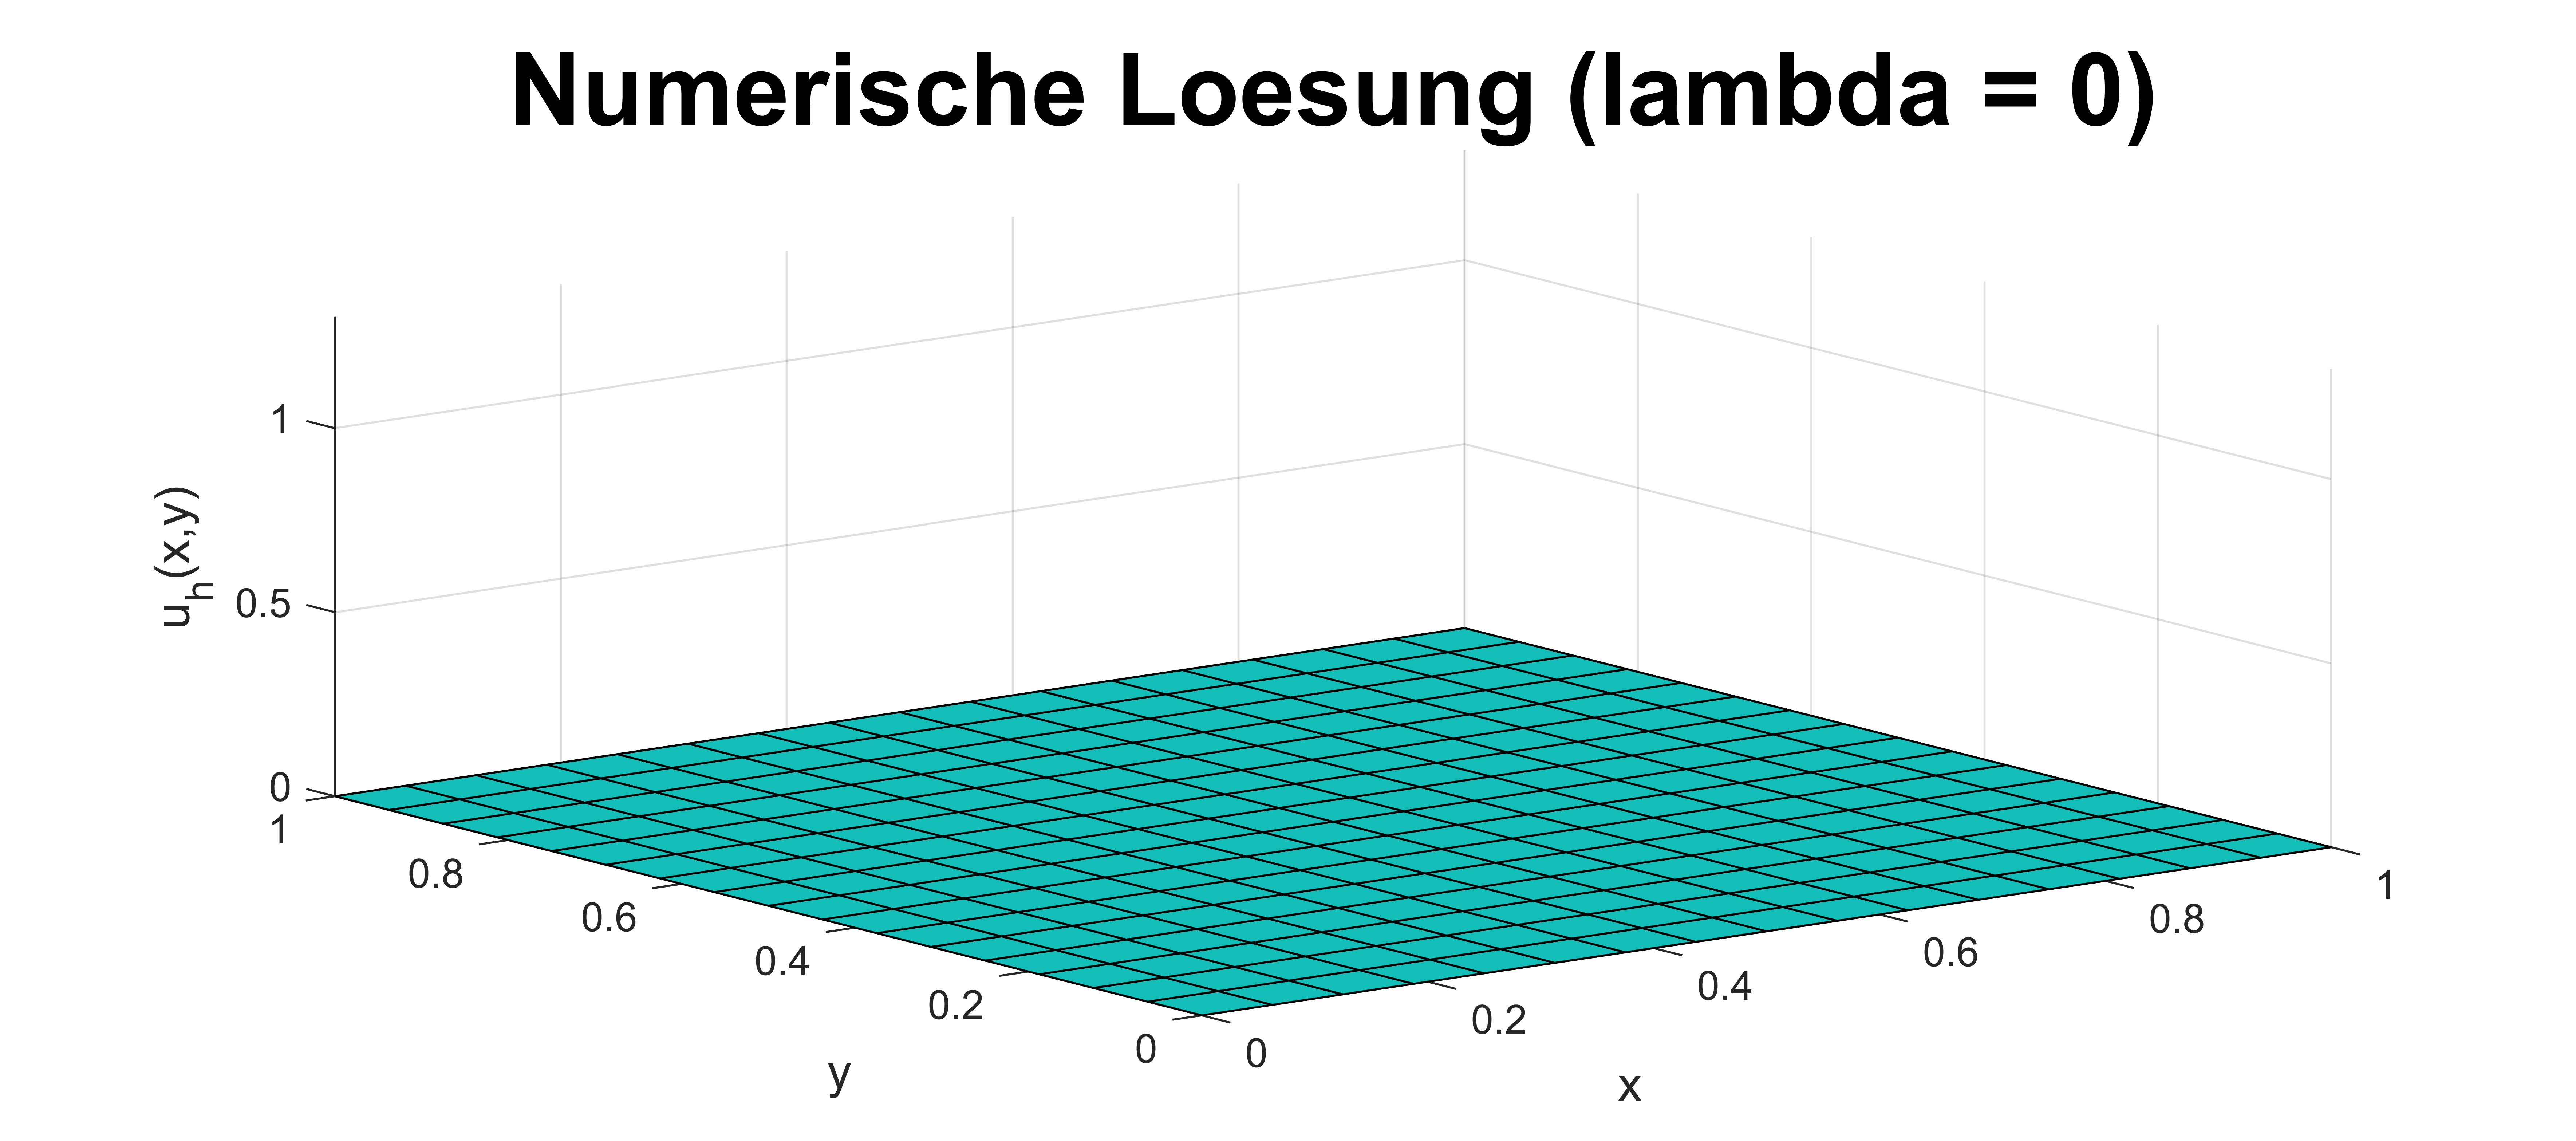
\includegraphics[width=0.3\textwidth]{bild2-0} &  
  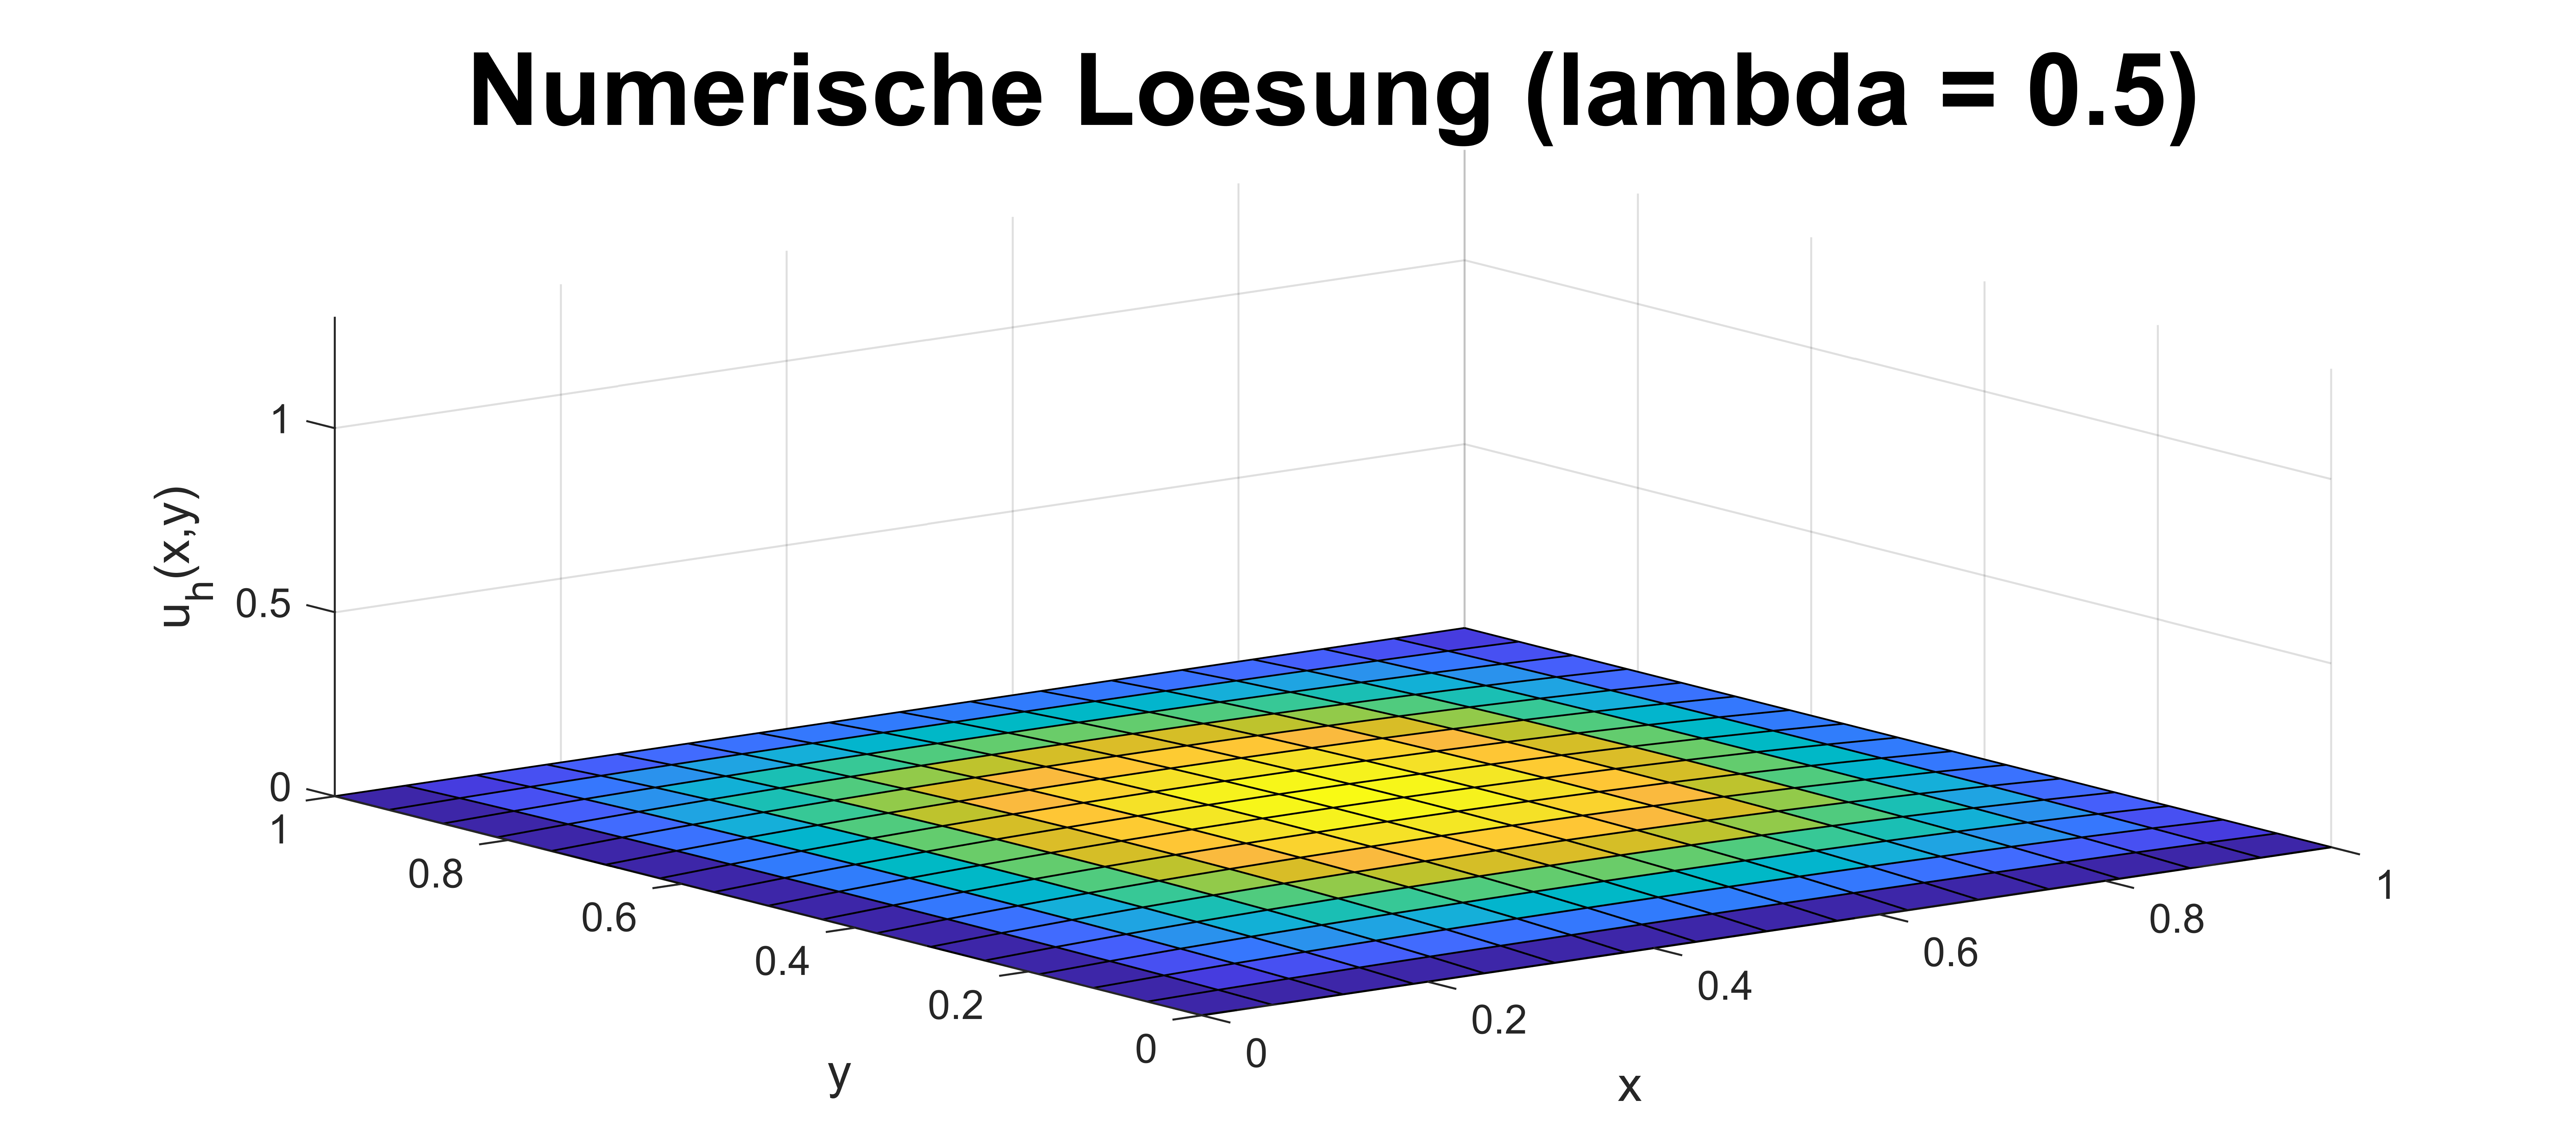
\includegraphics[width=0.3\textwidth]{bild2-0.5.png} &
  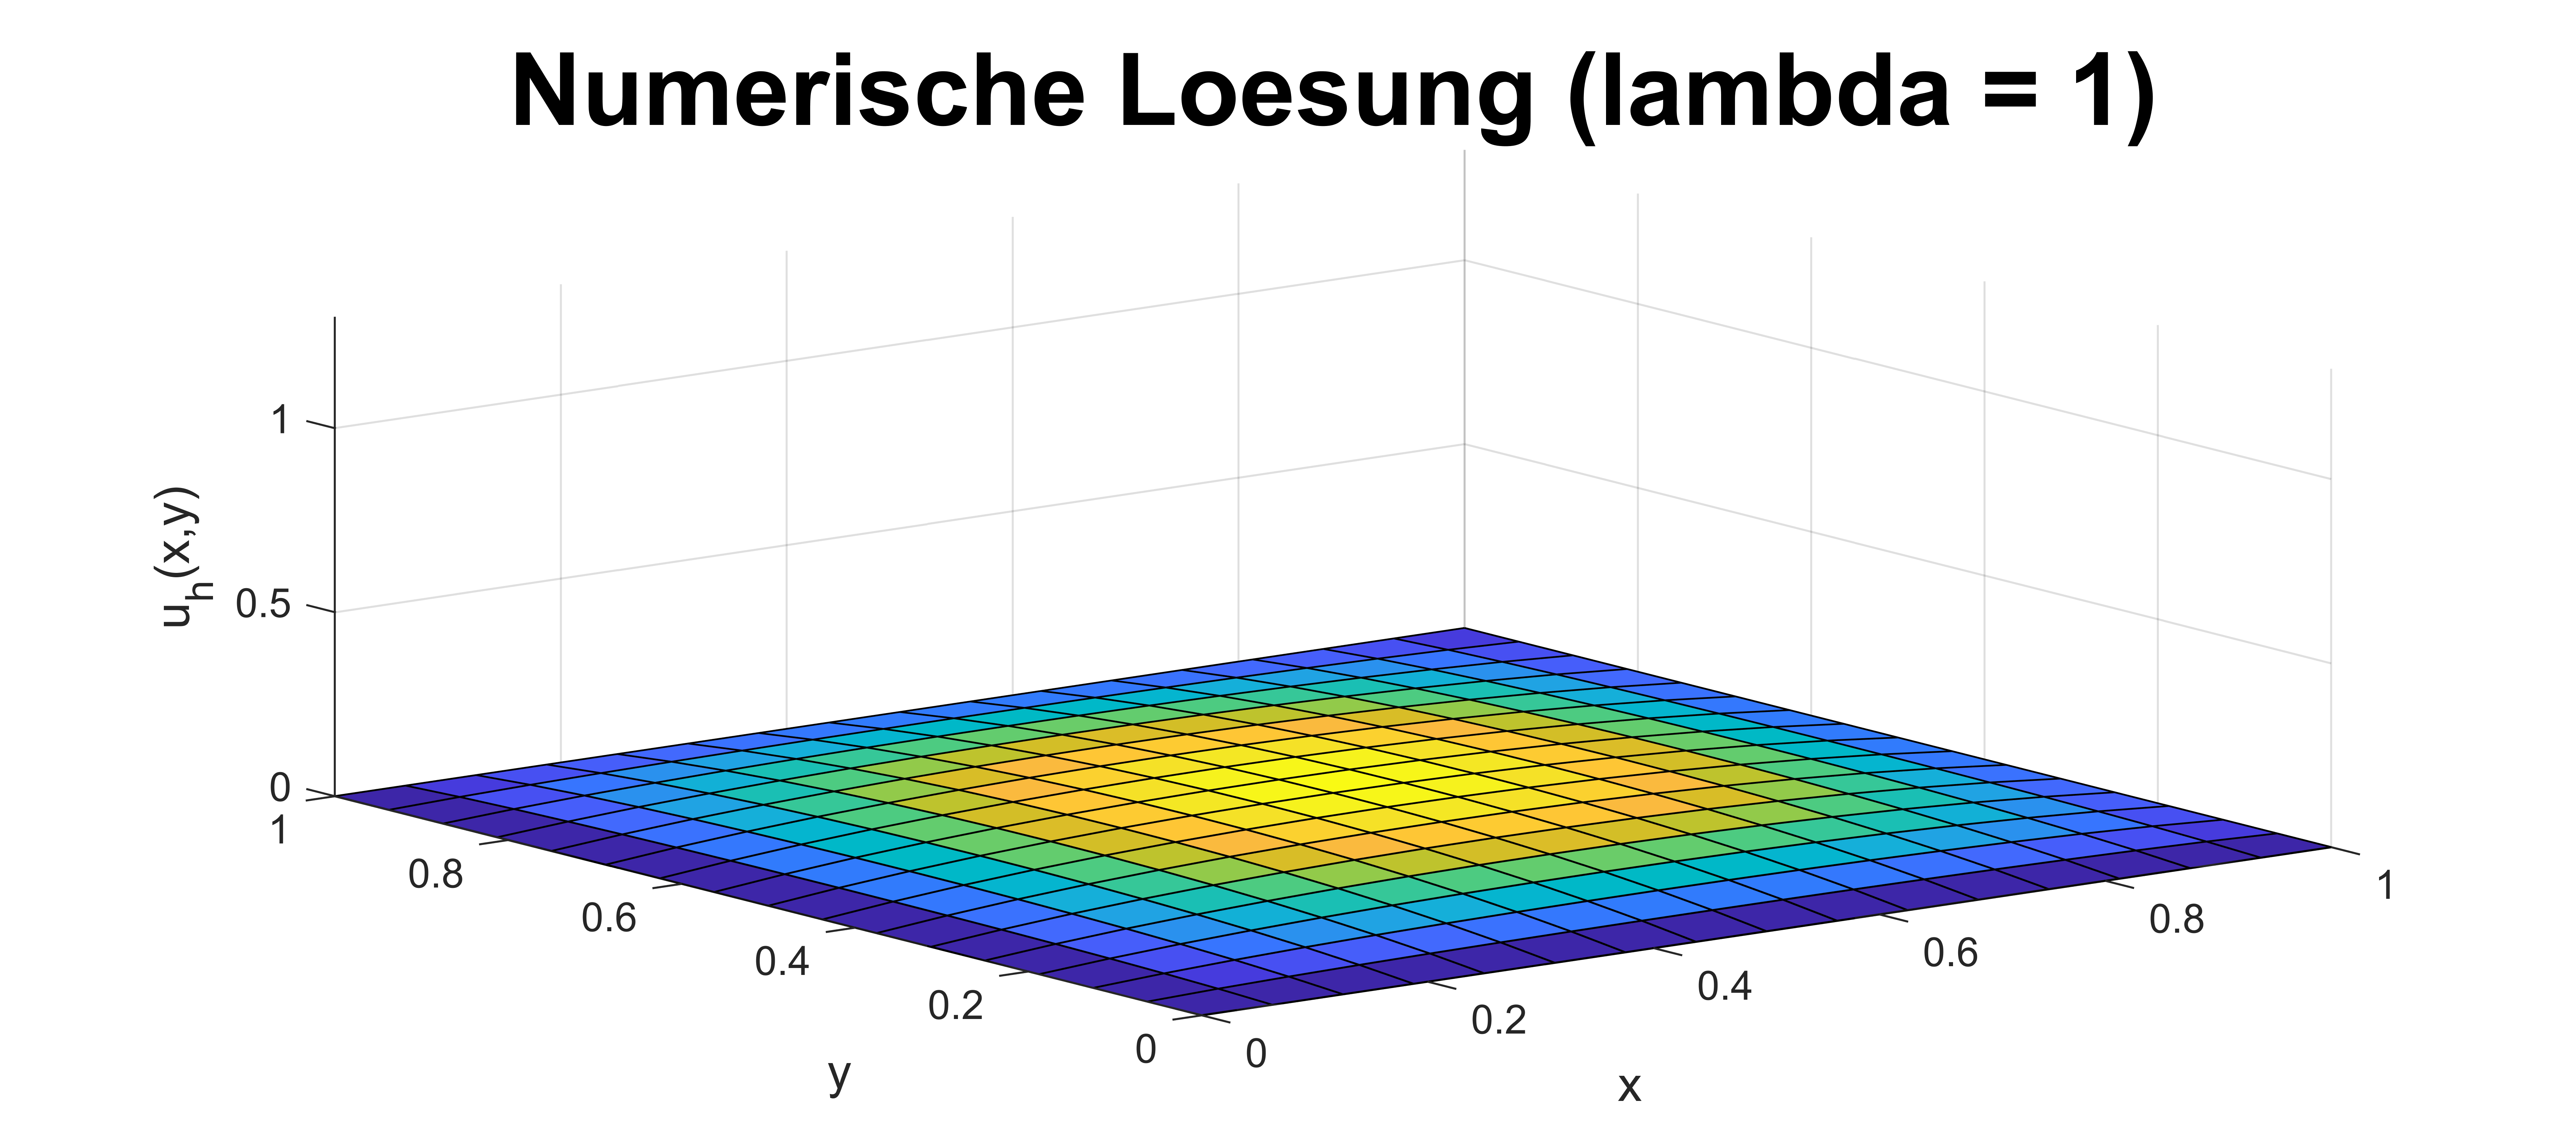
\includegraphics[width=0.3\textwidth]{bild2-1} \\
  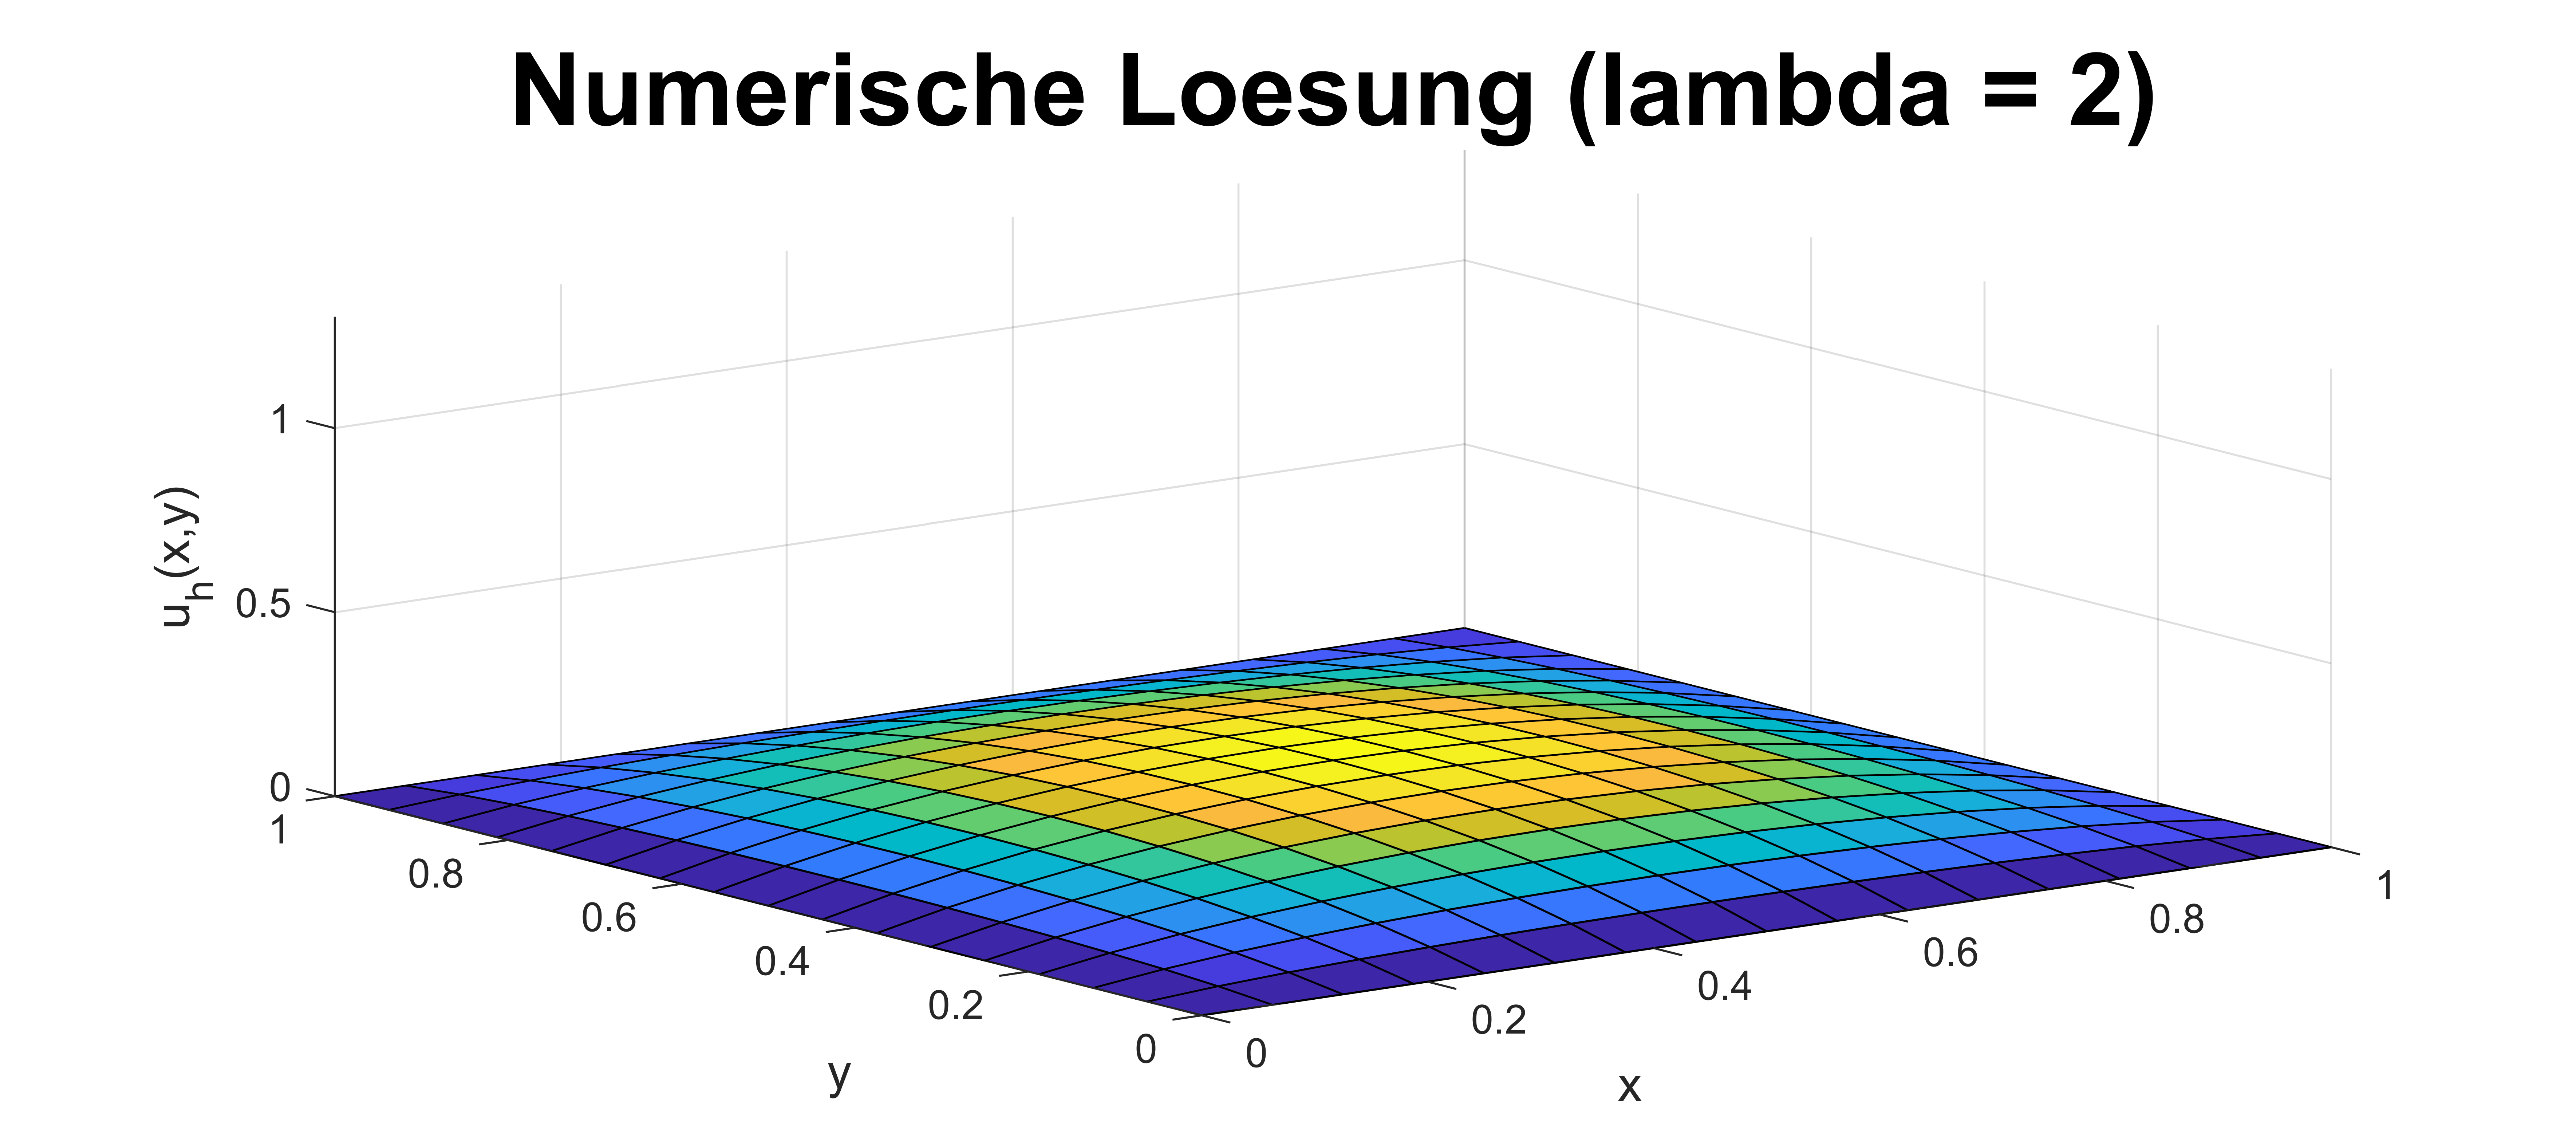
\includegraphics[width=0.3\textwidth]{bild2-2} &  
  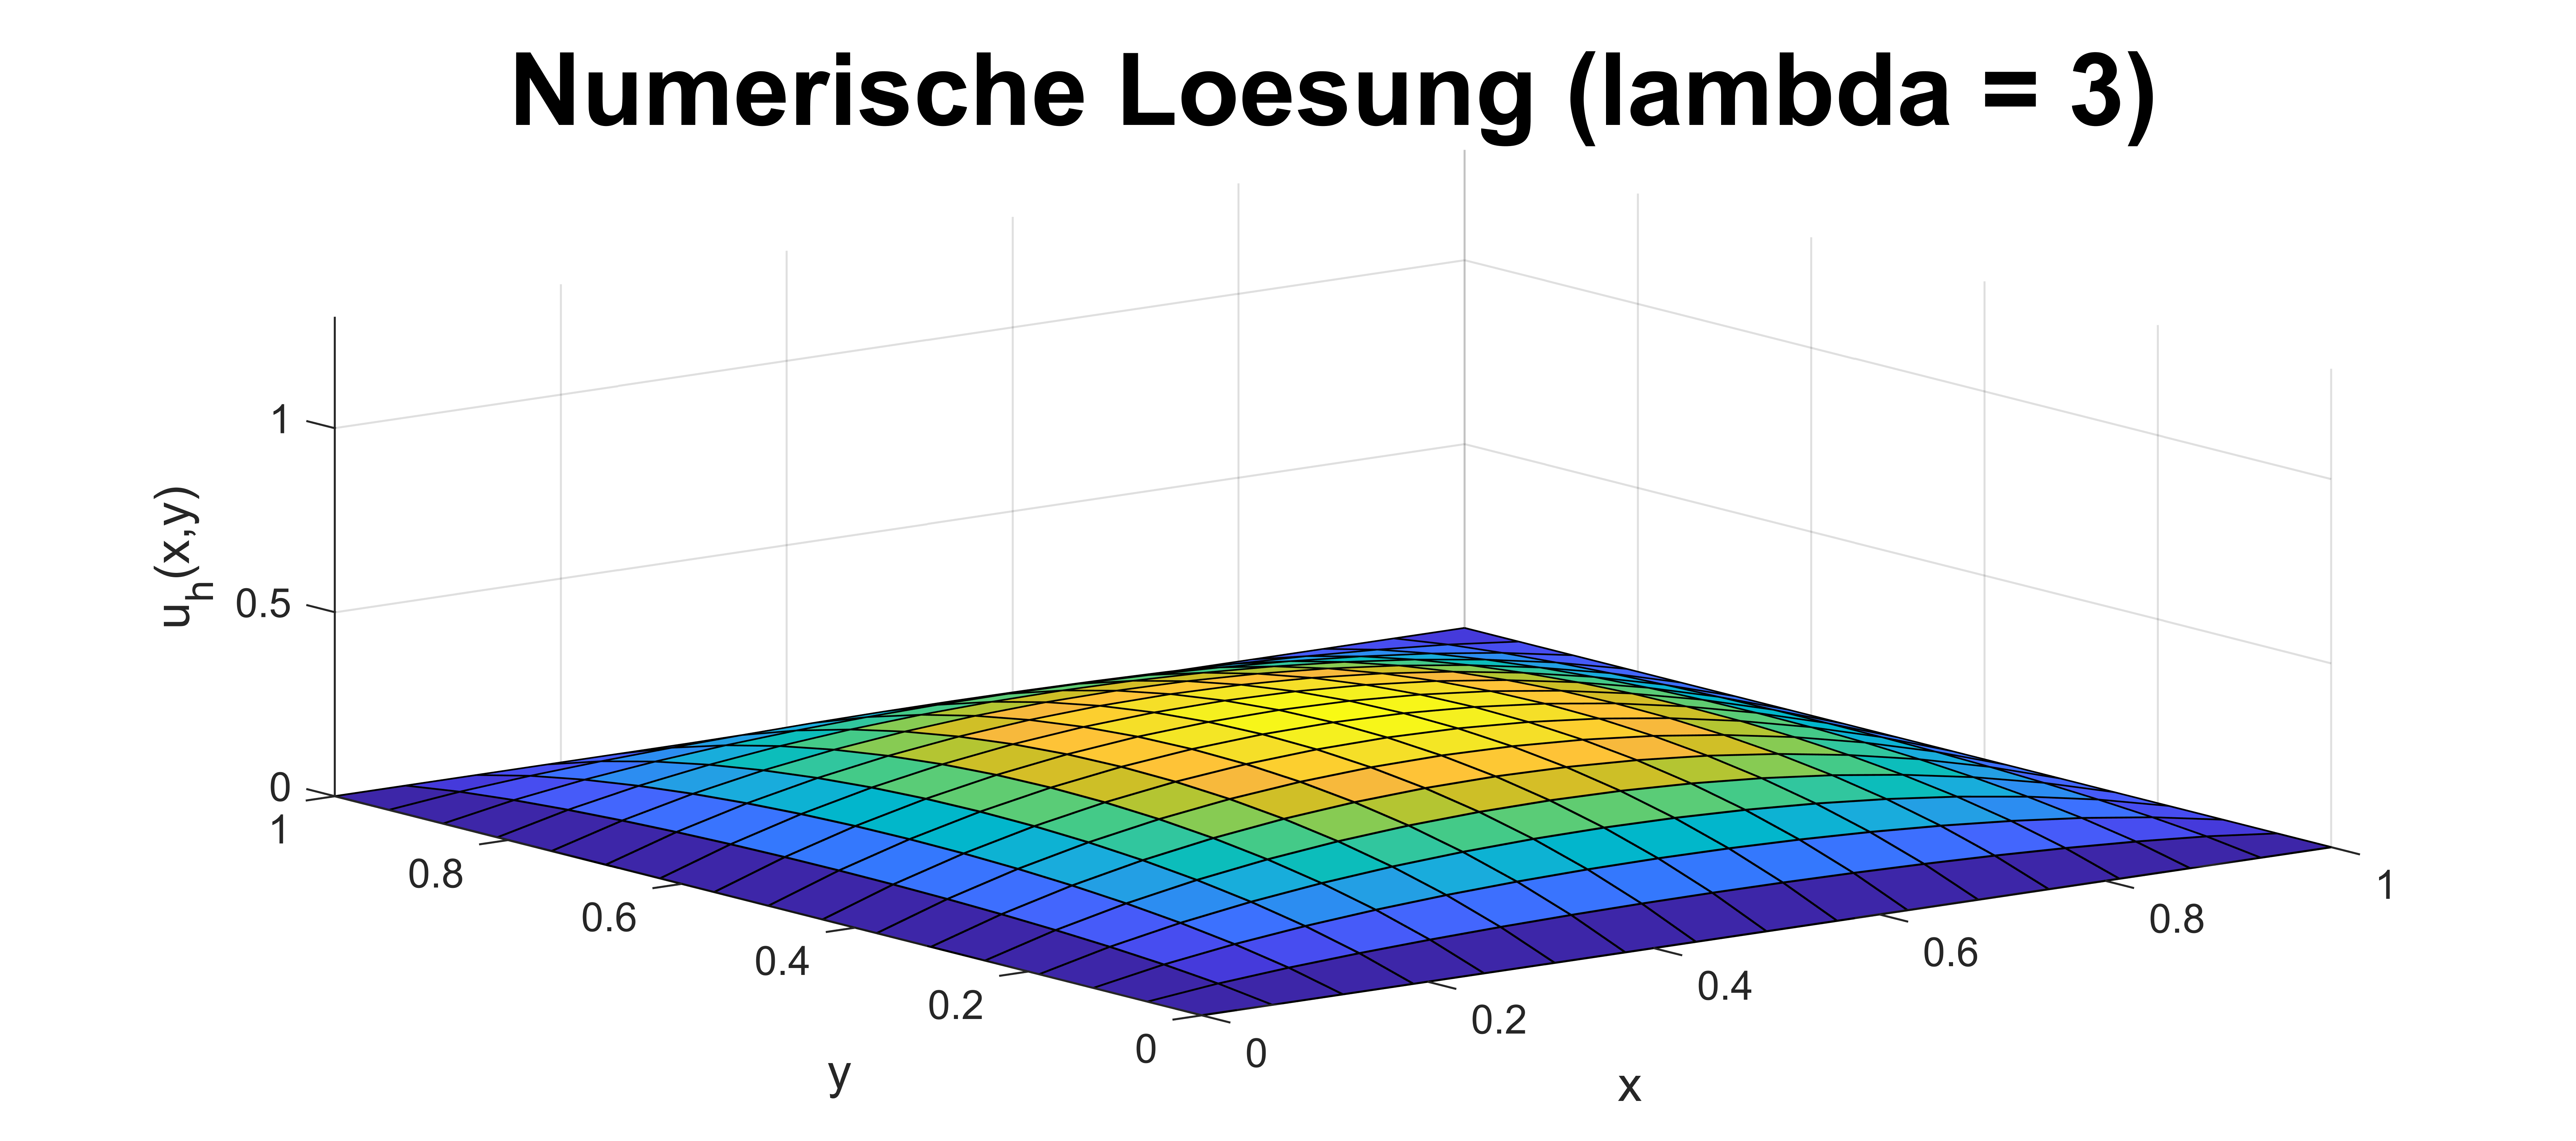
\includegraphics[width=0.3\textwidth]{bild2-3} &
  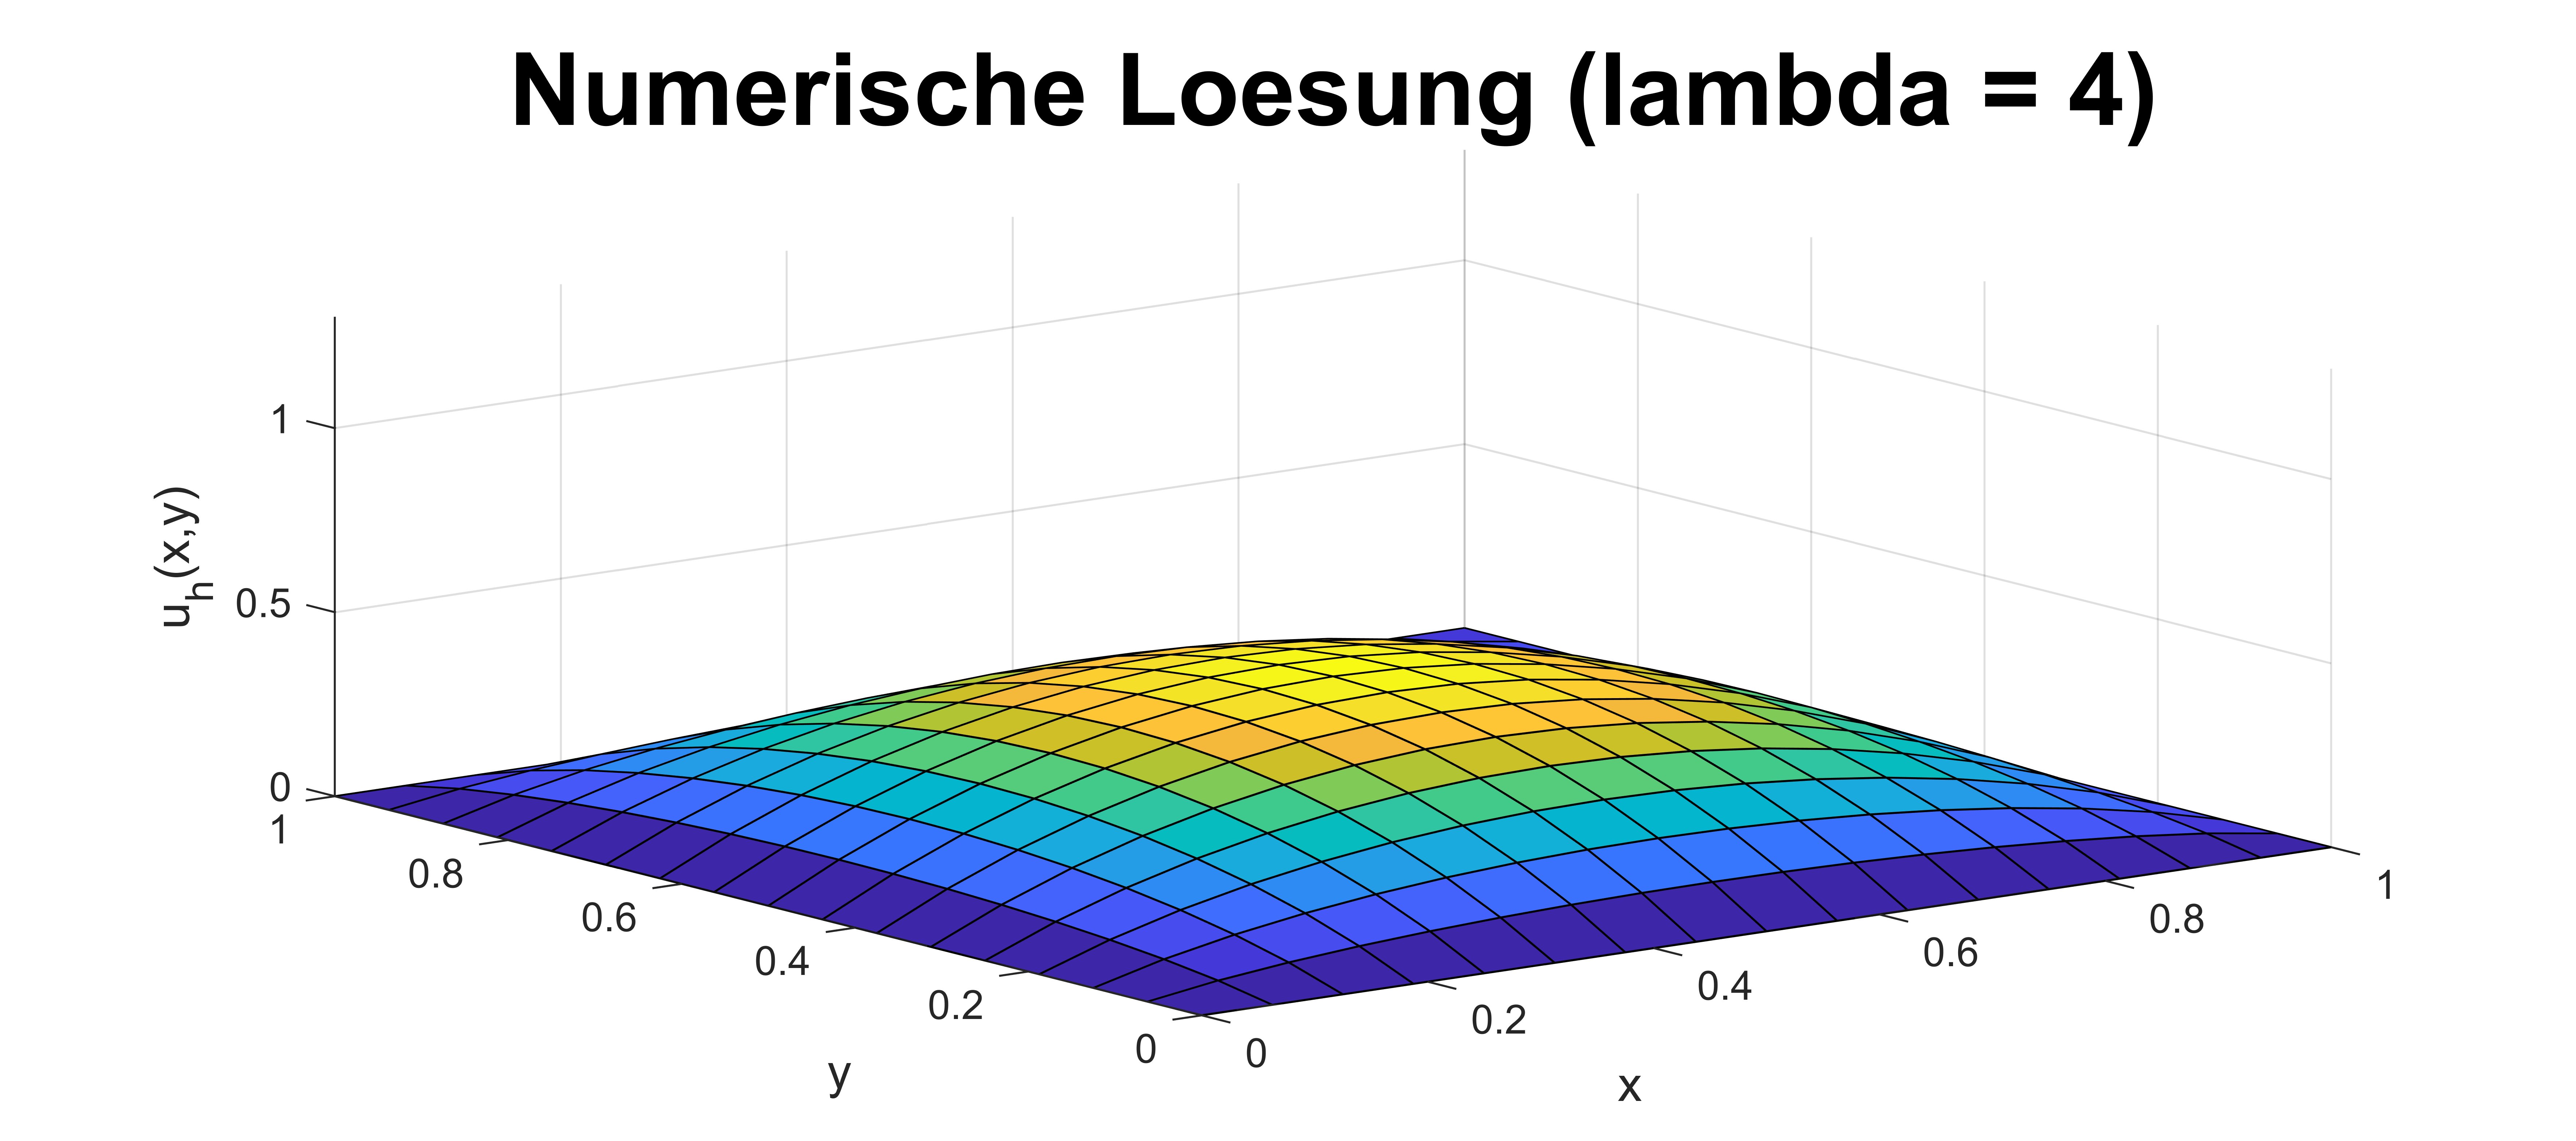
\includegraphics[width=0.3\textwidth]{bild2-4} \\
  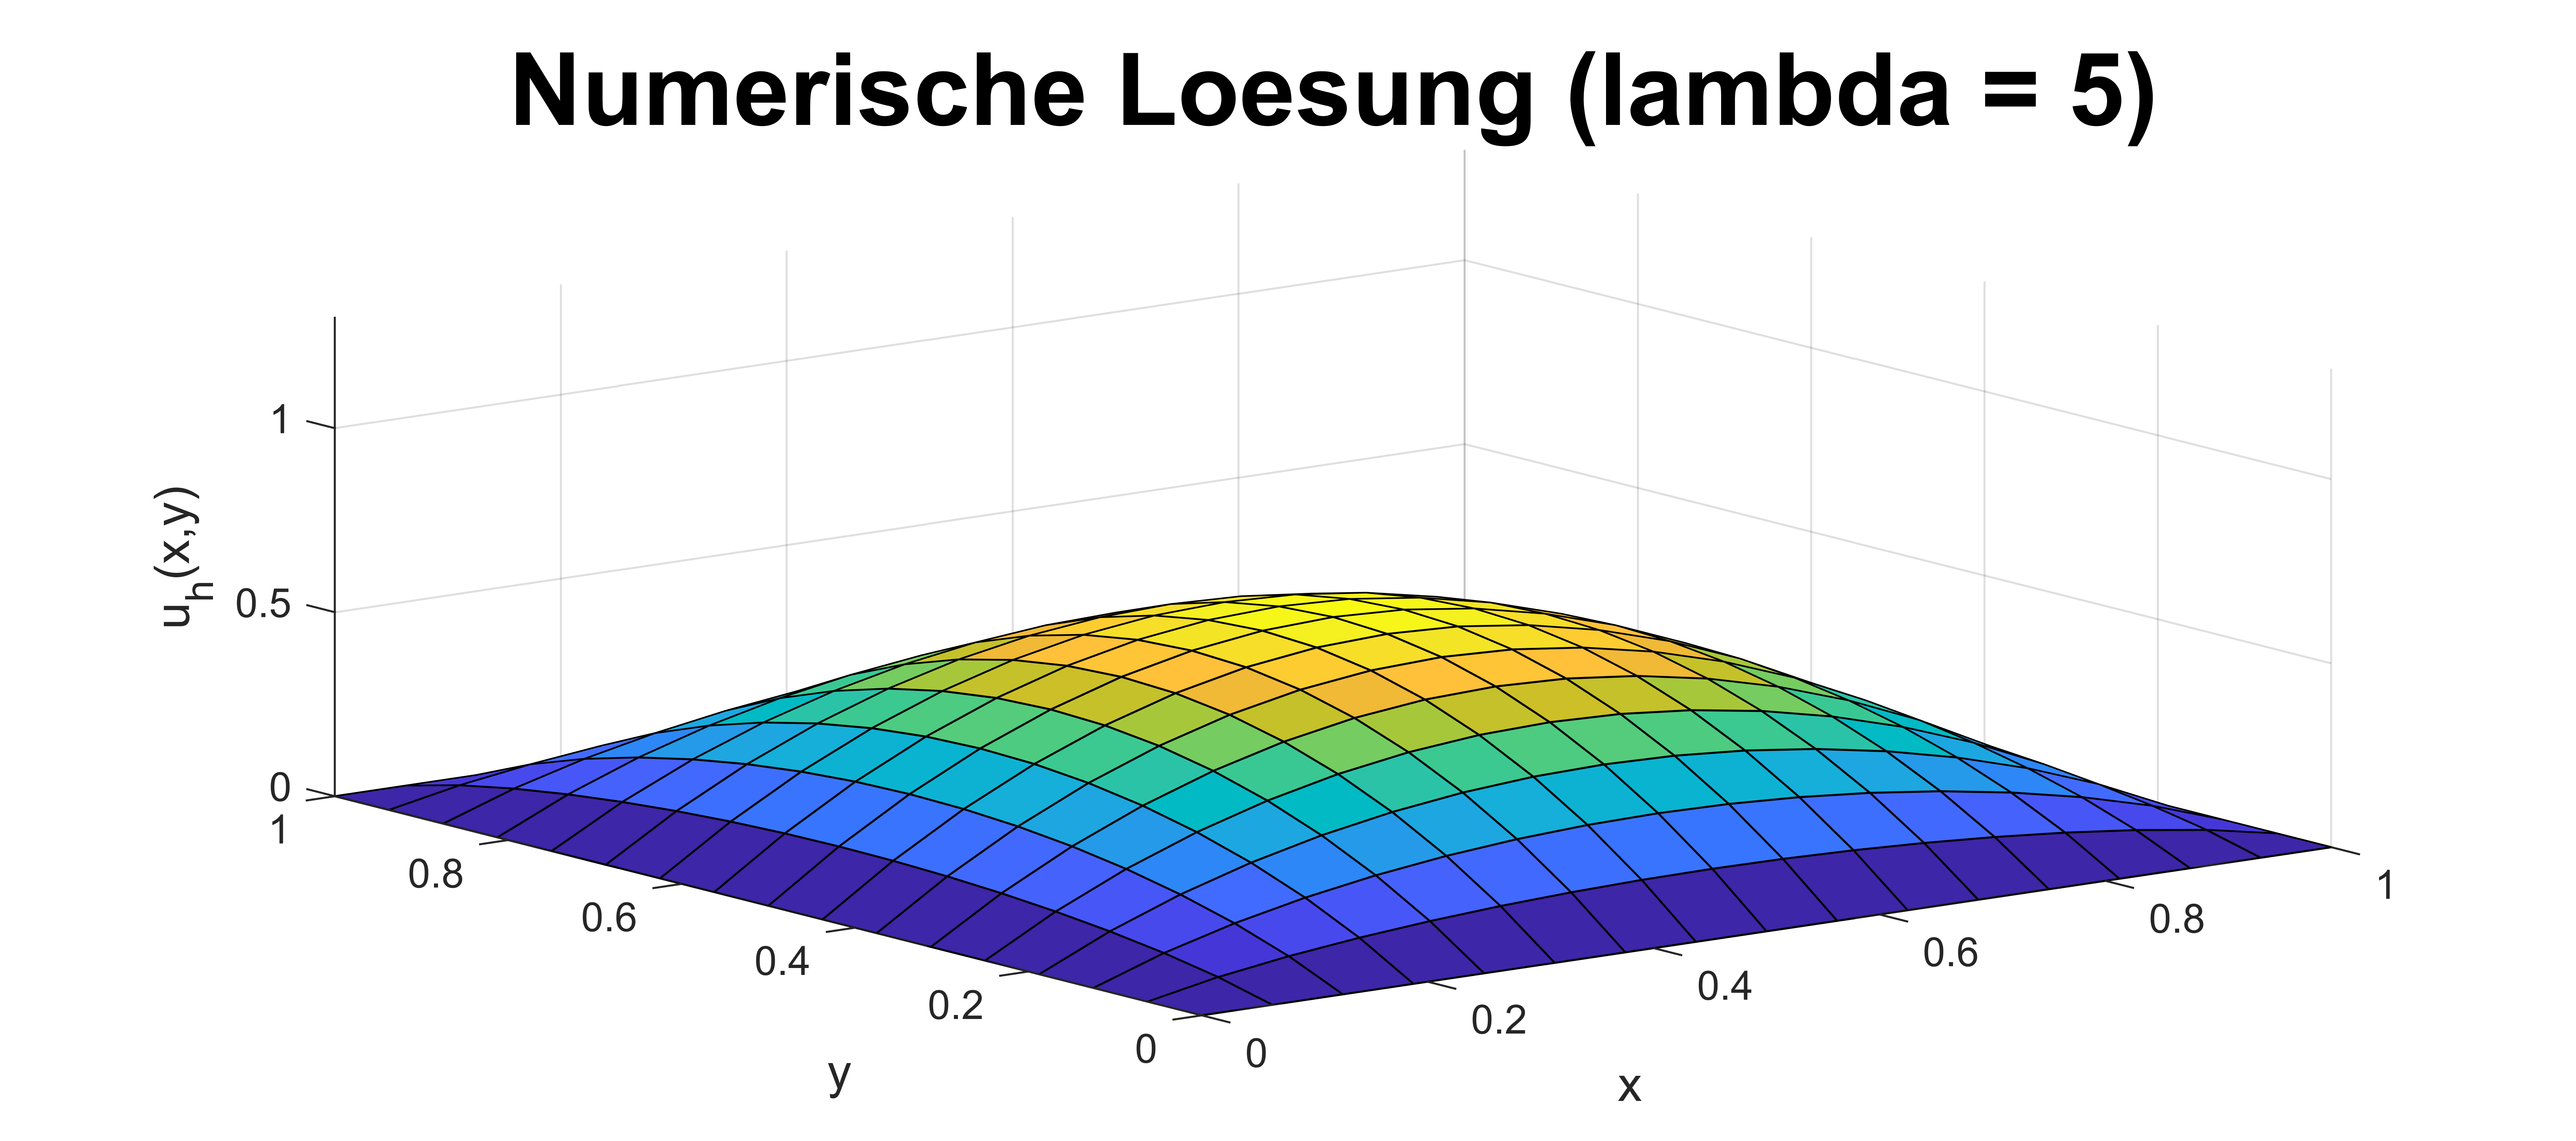
\includegraphics[width=0.3\textwidth]{bild2-5} &  
  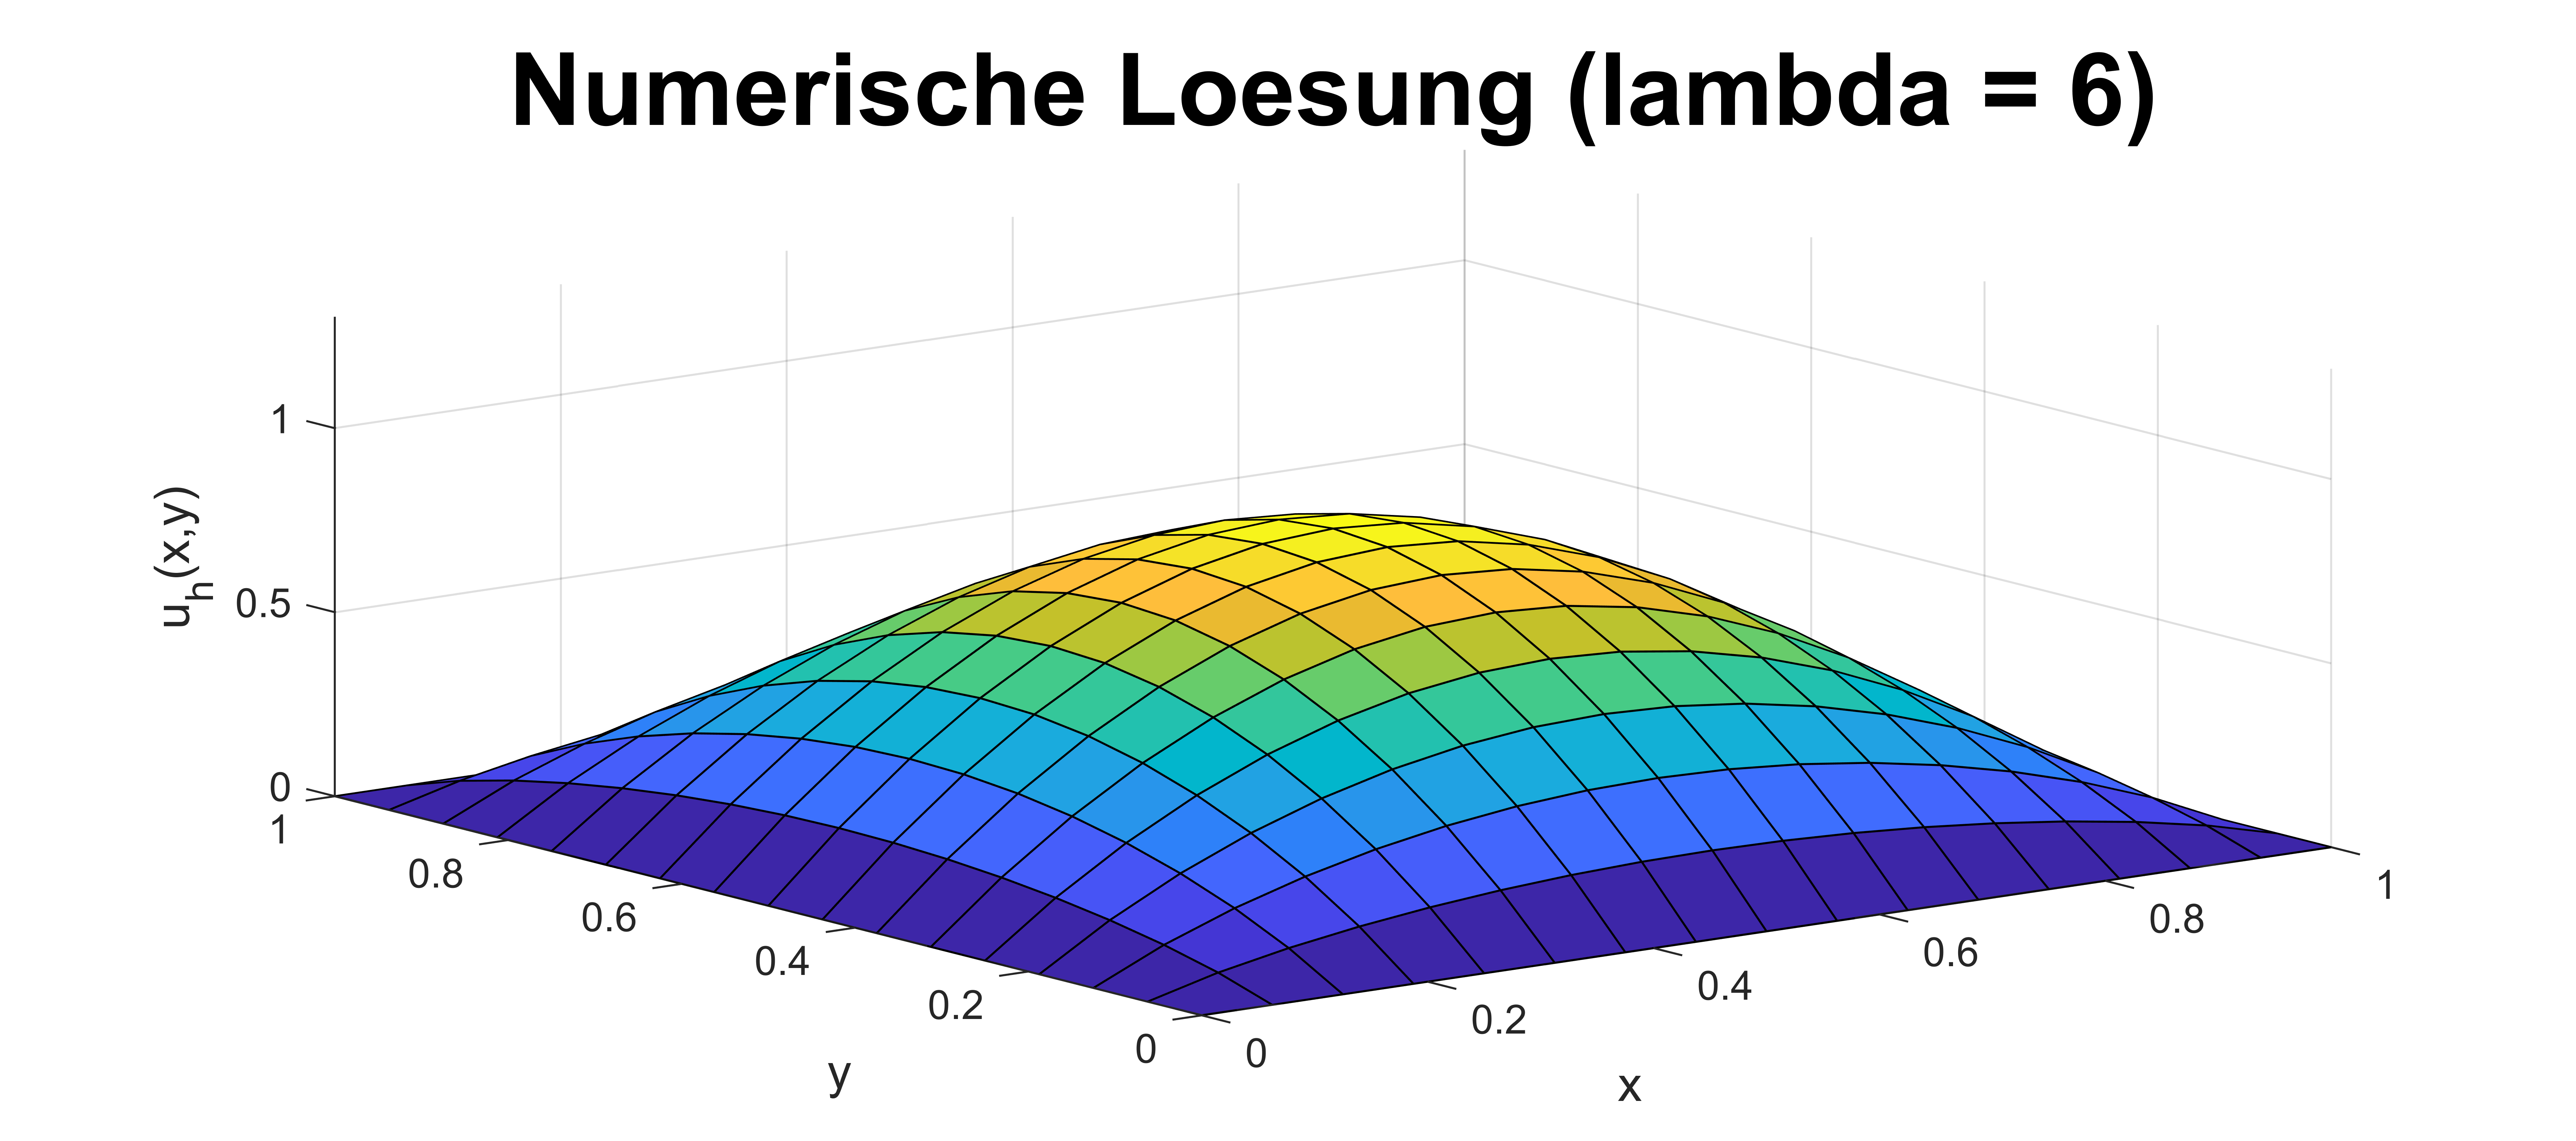
\includegraphics[width=0.3\textwidth]{bild2-6} &
  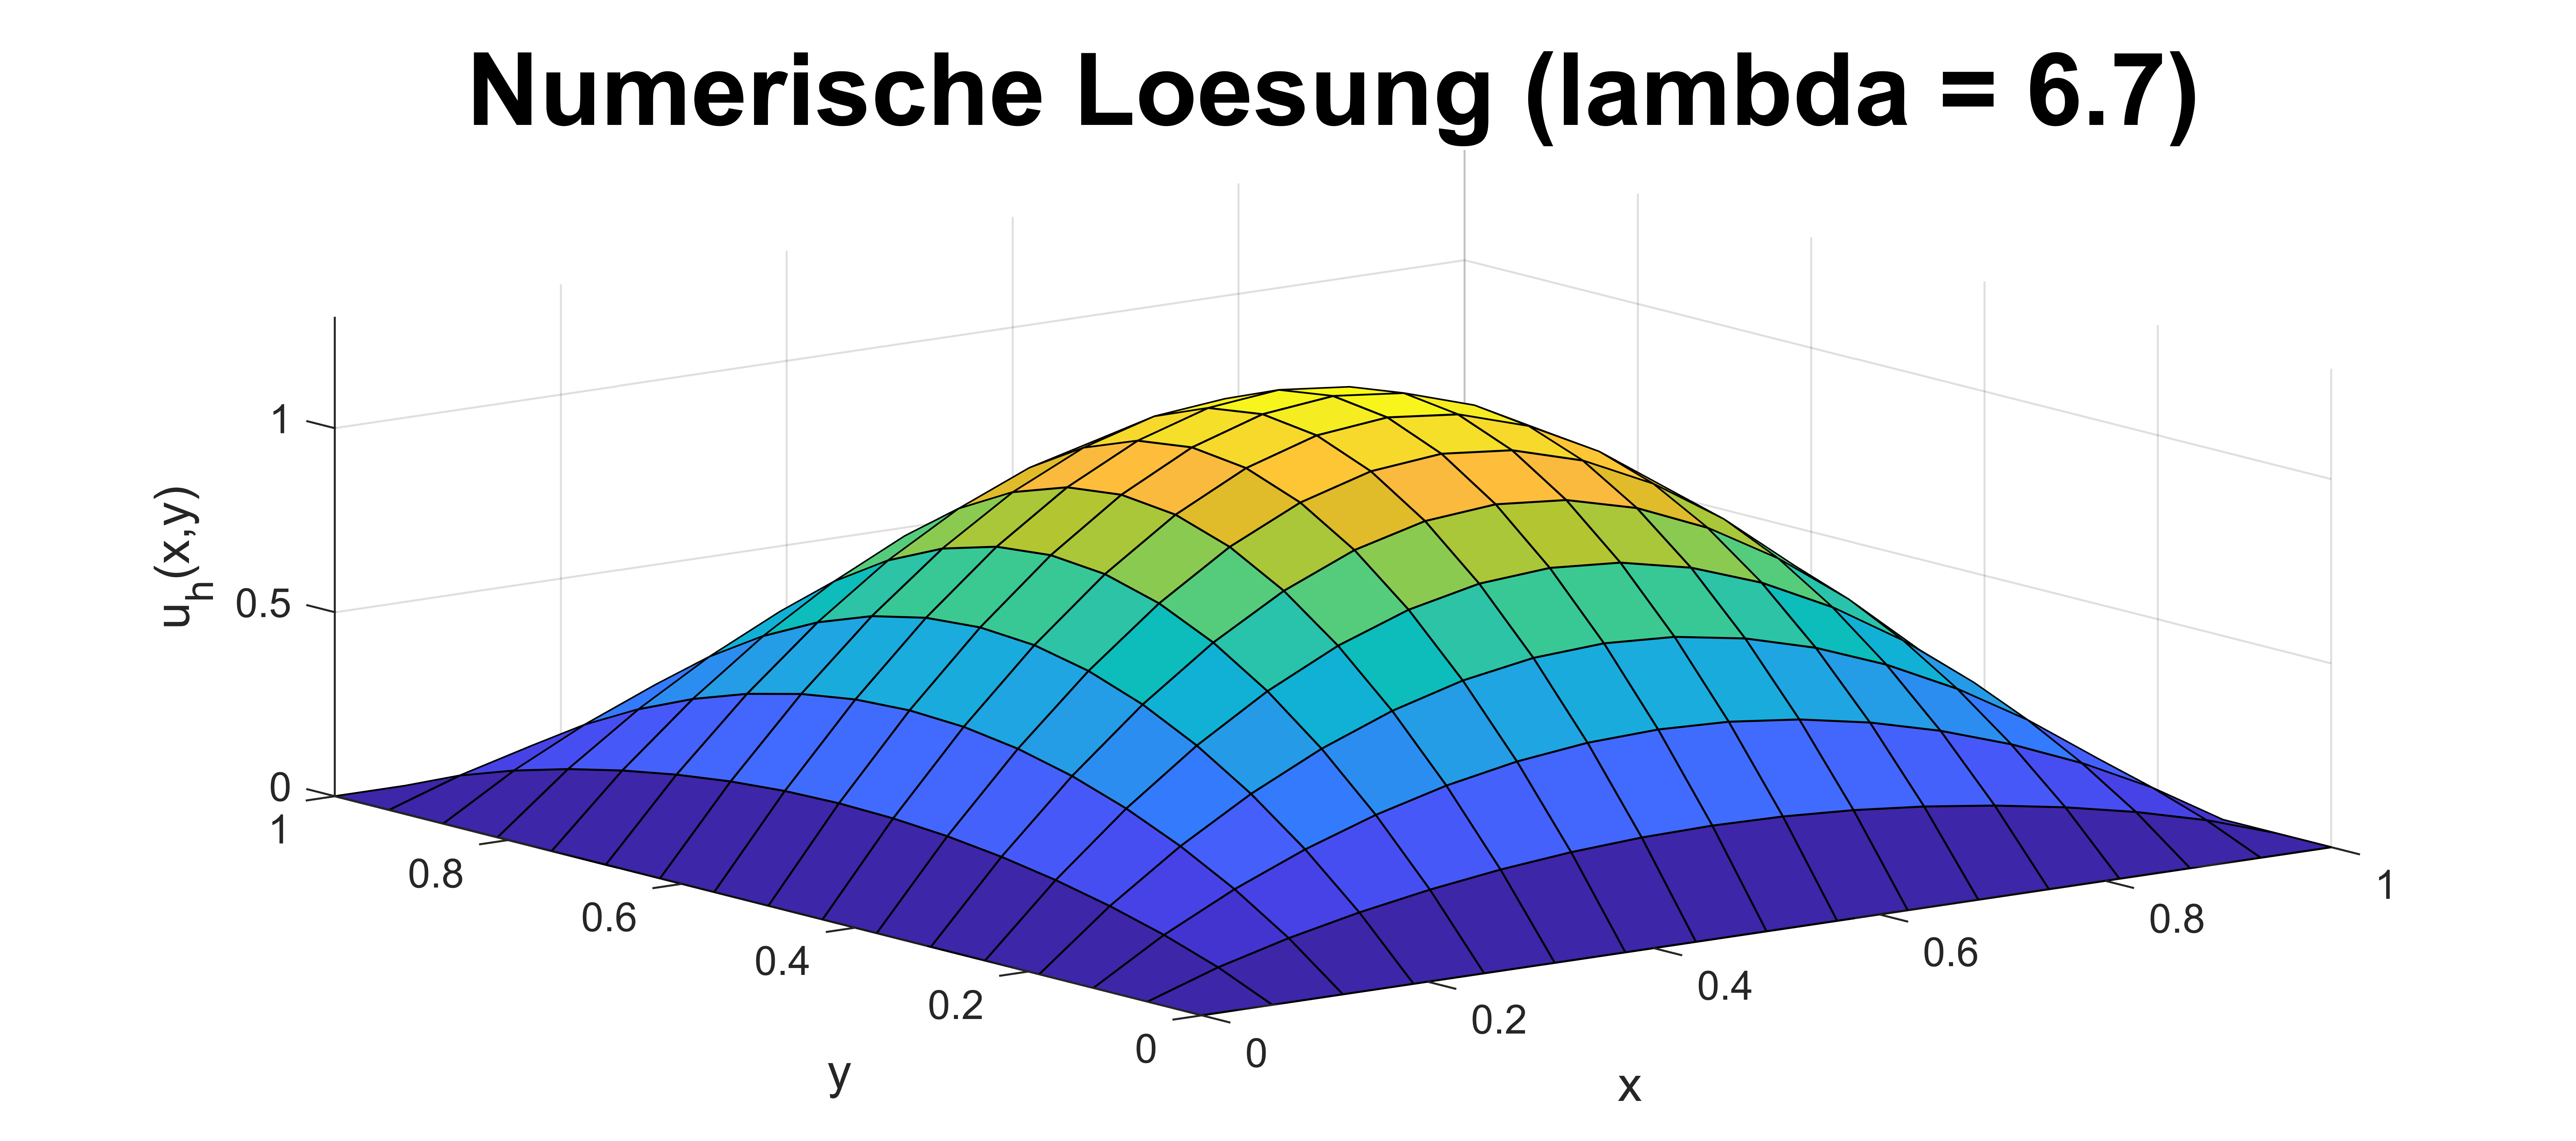
\includegraphics[width=0.3\textwidth]{bild2-6.7.png} \\
  
  \end{tabular}
\caption{Verlauf der numerischen L\"osung f\"ur gew\"ahlte $\lambda$}
  \end{figure}
  
Das Problem ist eine elliptische, partielle Differentialgleichung.\\
  
In Abbildung 1 sieht man den Verlauf der numerischen L\"osung.\\

In Abbildung 2 sieht man die Diskretisierung von $\Omega$.\\

Man betrachtet nun die $L-\infty$ Norm der numerischen L\"osung und trägt diese den das $\lambda$ in Abbildung 3 auf. Man sieht ein exponentielles Wachstum.

\begin{figure}
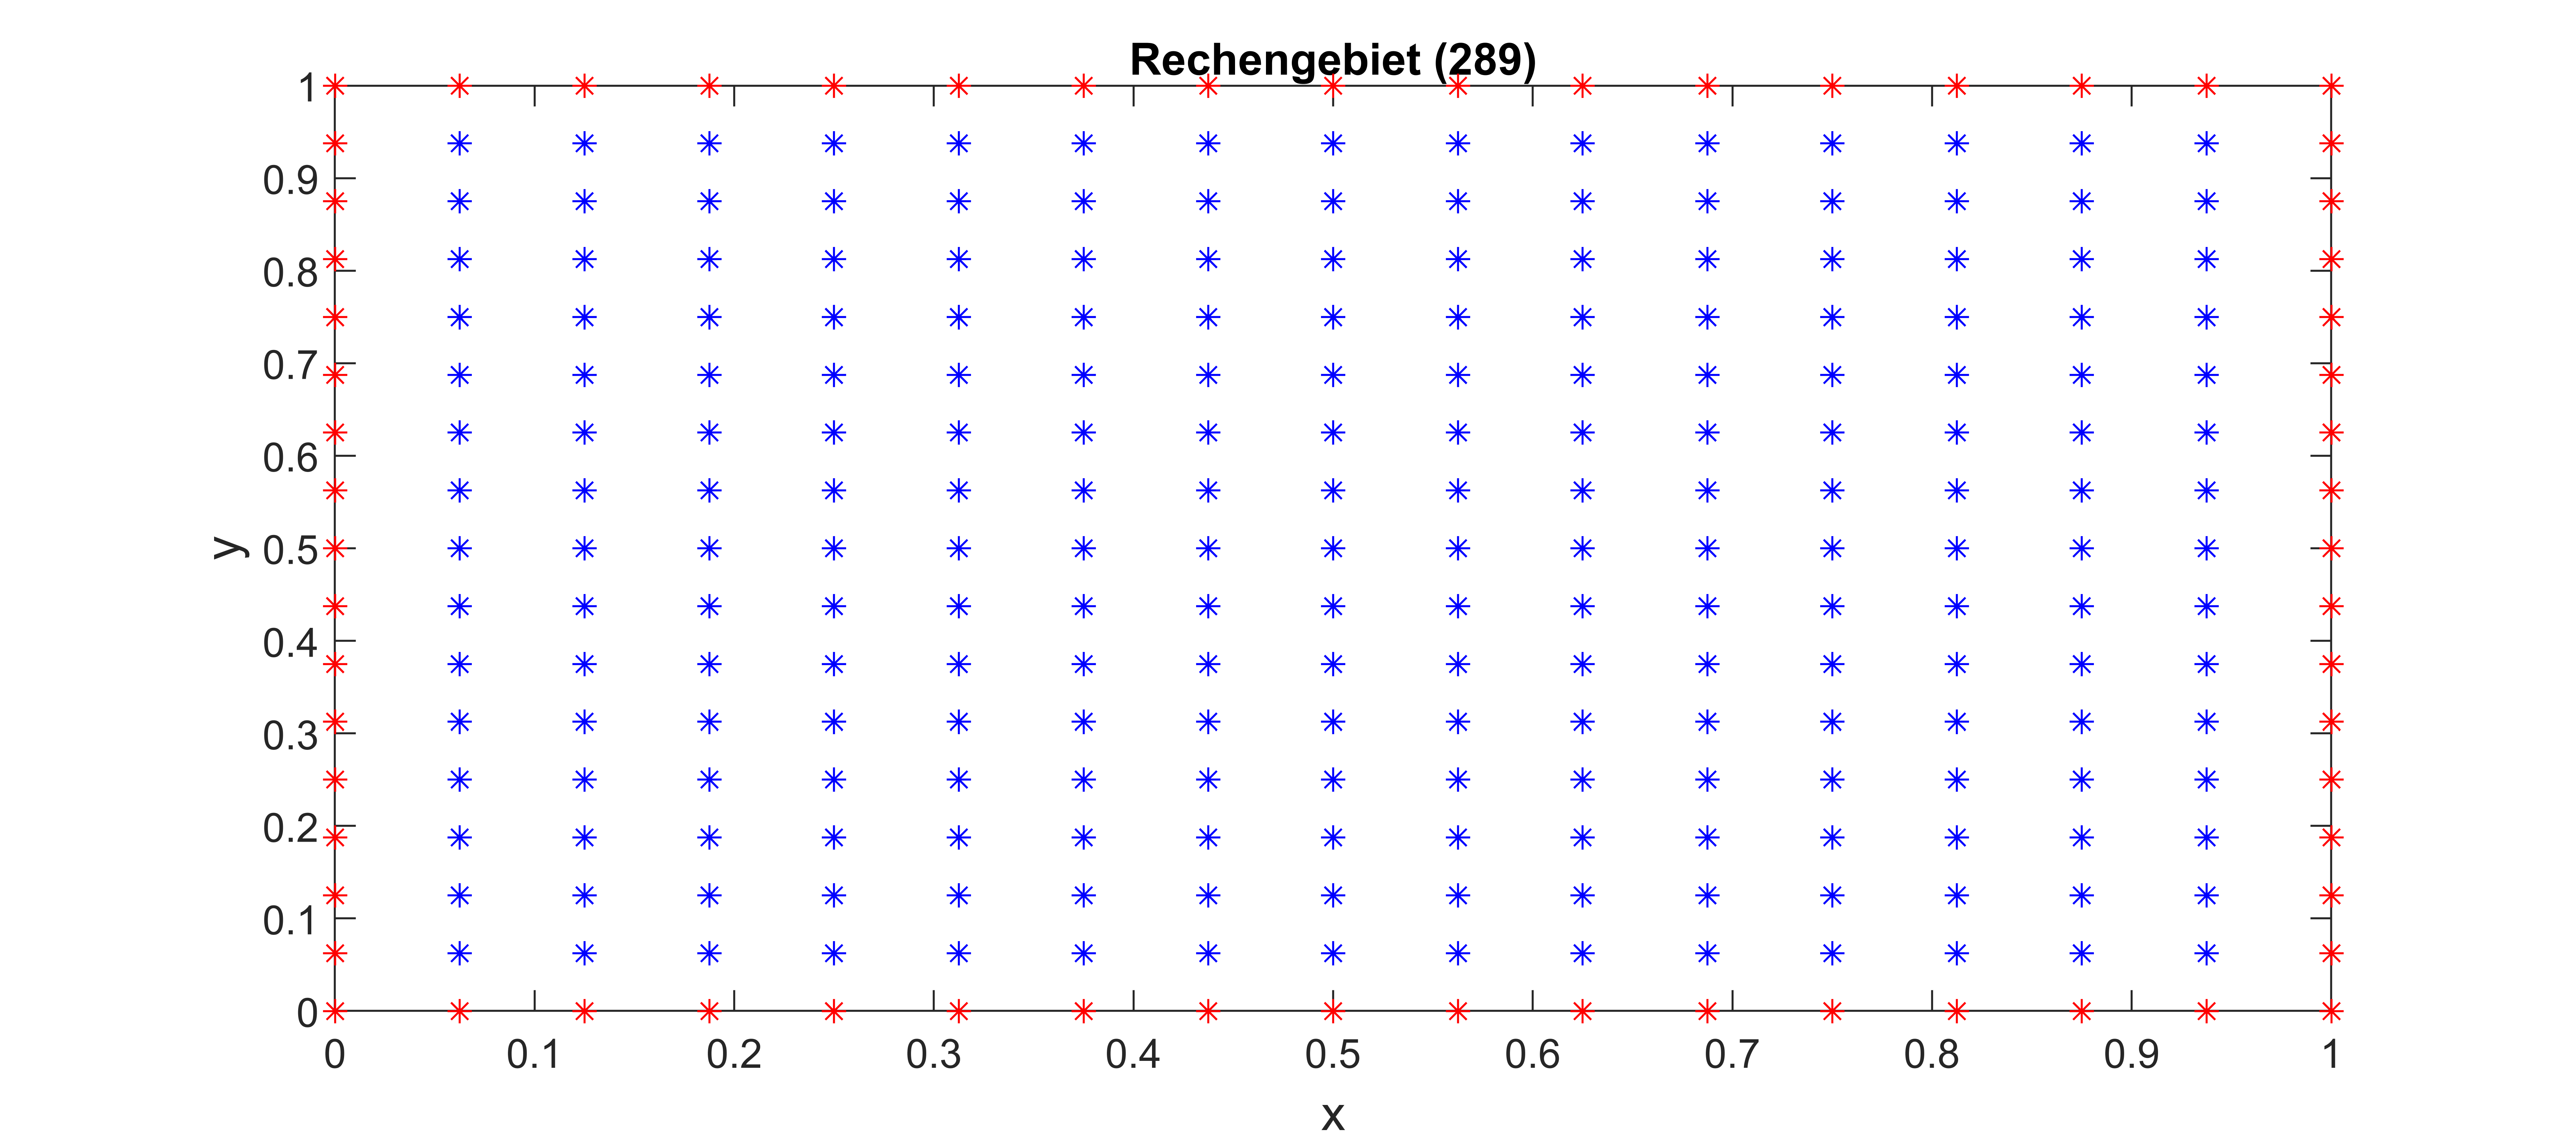
\includegraphics[width=0.8\textwidth]{bild1}
\caption{Diskretisierung von $\Omega$}
\end{figure}  


\begin{figure}
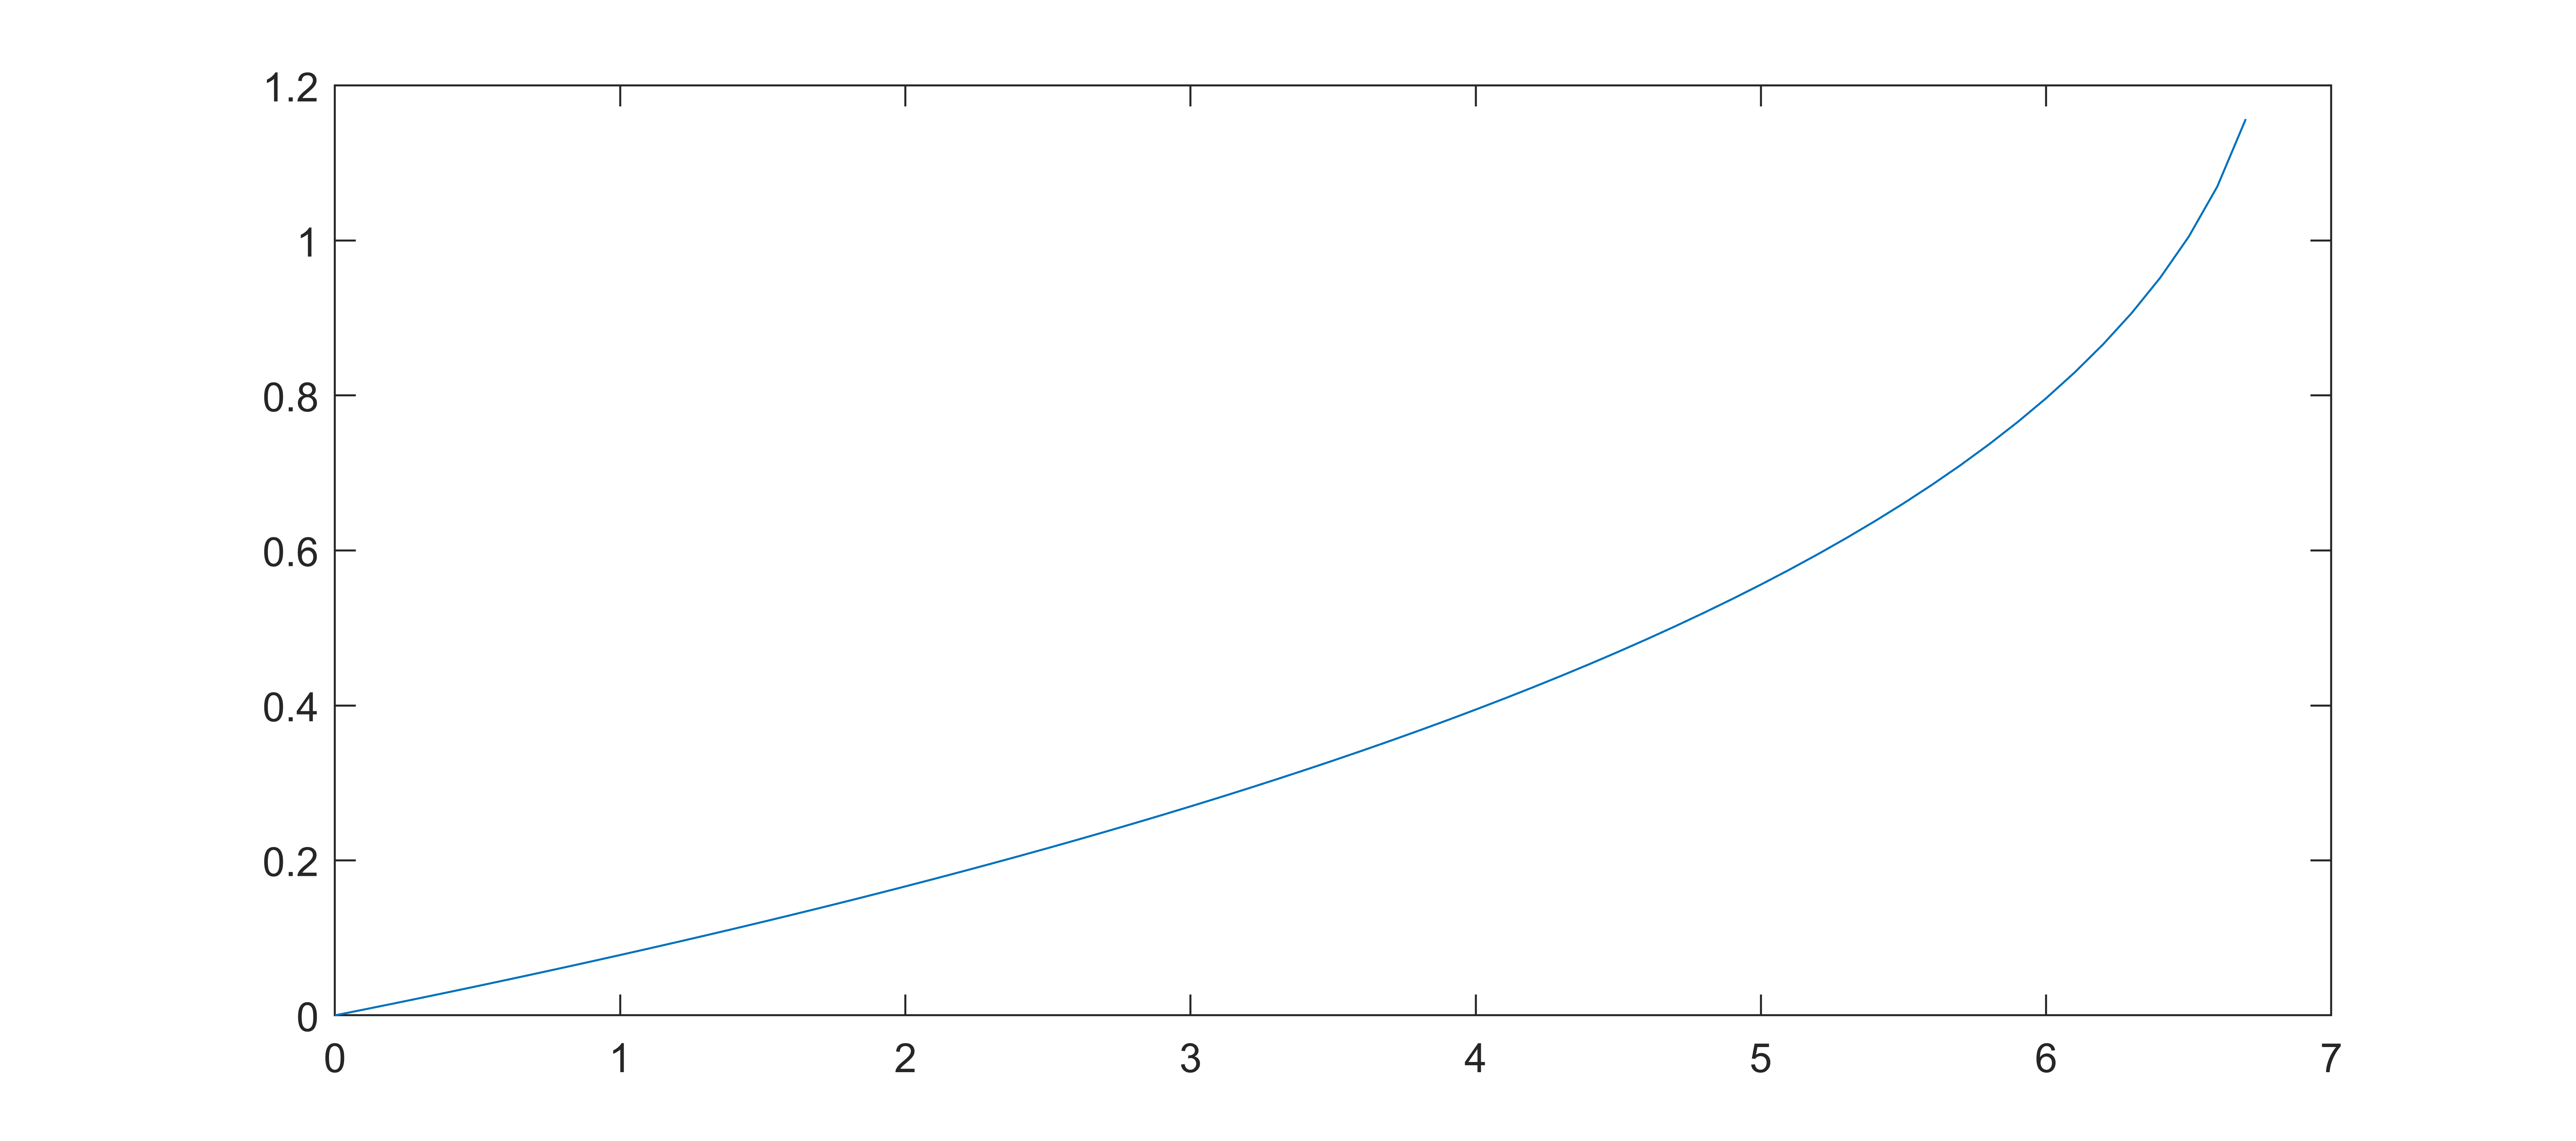
\includegraphics[width=0.8\textwidth]{bild3}
\caption{$L-\infty$ Norm der numerischen L\"osung aufgetragen gegen $lambda$}
\end{figure}  

\end{document}
